\documentclass[11pt,a4paper]{ctexart}
% Shared preamble for the assignment reports. Use with:
%   \documentclass[11pt,a4paper]{ctexart}  (XeLaTeX)
%   % Shared preamble for the assignment reports. Use with:
%   \documentclass[11pt,a4paper]{ctexart}  (XeLaTeX)
%   % Shared preamble for the assignment reports. Use with:
%   \documentclass[11pt,a4paper]{ctexart}  (XeLaTeX)
%   \input{../common/preamble.tex}
\usepackage[margin=2.3cm]{geometry}
\setmainfont{texgyretermes}[Extension=.otf,UprightFont=*-regular,BoldFont=*-bold,ItalicFont=*-italic,BoldItalicFont=*-bolditalic]
\setsansfont{texgyreheros}[Extension=.otf,UprightFont=*-regular,BoldFont=*-bold,ItalicFont=*-italic,BoldItalicFont=*-bolditalic]
\setmonofont{texgyrecursor}[Extension=.otf,UprightFont=*-regular,BoldFont=*-bold,ItalicFont=*-italic,BoldItalicFont=*-bolditalic]
\usepackage{amsmath,amssymb,mathtools,bm}
\usepackage{graphicx}
\usepackage{booktabs,multirow,makecell,array,tabularx}
\usepackage[table]{xcolor}
\usepackage[most]{tcolorbox}
\usepackage{enumitem}
\usepackage{listings}
\usepackage{subcaption}
\usepackage{siunitx}
\usepackage[hidelinks]{hyperref}
\usepackage[nameinlink,noabbrev]{cleveref}
\usepackage{float}

\setlength{\emergencystretch}{3em}
\linespread{1.15}
\setlist{leftmargin=*,itemsep=2pt,topsep=3pt}
\graphicspath{{figures/}}

\crefname{figure}{图}{图}
\crefname{table}{表}{表}
\crefname{section}{第}{第}
\creflabelformat{section}{#2#1#3 节}
\crefname{equation}{式}{式}
\crefformat{equation}{式~(#2#1#3)}

\lstset{basicstyle=\ttfamily\footnotesize,columns=fullflexible,breaklines=true,frame=single,
  framerule=0.3pt,rulecolor=\color{black!40},backgroundcolor=\color{black!3},
  keywordstyle=\color{blue!60!black}\bfseries,commentstyle=\color{green!40!black},
  numbers=left,numberstyle=\tiny\color{black!50},xleftmargin=1.5em}

% Interview boxes: question, model answer, common wrong answer.
\newtcolorbox{iqbox}[1]{enhanced,breakable,colback=blue!3,colframe=blue!45!black,boxrule=0.5pt,arc=1.5pt,
  left=4pt,right=4pt,top=3pt,bottom=3pt,fonttitle=\bfseries\small,title={面试追问：#1}}
\newtcolorbox{findingbox}[1][]{enhanced,breakable,colback=green!3,colframe=green!40!black,boxrule=0.5pt,arc=1.5pt,
  left=4pt,right=4pt,top=3pt,bottom=3pt,fonttitle=\bfseries\small,title={结论#1}}
\newtcolorbox{caveatbox}{enhanced,breakable,colback=orange!4,colframe=orange!60!black,boxrule=0.5pt,arc=1.5pt,
  left=4pt,right=4pt,top=3pt,bottom=3pt,fonttitle=\bfseries\small,title={不能推出的结论}}

\newcommand{\authorline}{ShaneLiu04\thanks{GitHub: \url{https://github.com/ShaneLiu04}。代码与原始指标见 edge-deploy 仓库各 lab 的 \texttt{artifacts/raw/}。本文基于公开课程材料独立完成，与课程团队无隶属关系。}}

\usepackage[margin=2.3cm]{geometry}
\setmainfont{texgyretermes}[Extension=.otf,UprightFont=*-regular,BoldFont=*-bold,ItalicFont=*-italic,BoldItalicFont=*-bolditalic]
\setsansfont{texgyreheros}[Extension=.otf,UprightFont=*-regular,BoldFont=*-bold,ItalicFont=*-italic,BoldItalicFont=*-bolditalic]
\setmonofont{texgyrecursor}[Extension=.otf,UprightFont=*-regular,BoldFont=*-bold,ItalicFont=*-italic,BoldItalicFont=*-bolditalic]
\usepackage{amsmath,amssymb,mathtools,bm}
\usepackage{graphicx}
\usepackage{booktabs,multirow,makecell,array,tabularx}
\usepackage[table]{xcolor}
\usepackage[most]{tcolorbox}
\usepackage{enumitem}
\usepackage{listings}
\usepackage{subcaption}
\usepackage{siunitx}
\usepackage[hidelinks]{hyperref}
\usepackage[nameinlink,noabbrev]{cleveref}
\usepackage{float}

\setlength{\emergencystretch}{3em}
\linespread{1.15}
\setlist{leftmargin=*,itemsep=2pt,topsep=3pt}
\graphicspath{{figures/}}

\crefname{figure}{图}{图}
\crefname{table}{表}{表}
\crefname{section}{第}{第}
\creflabelformat{section}{#2#1#3 节}
\crefname{equation}{式}{式}
\crefformat{equation}{式~(#2#1#3)}

\lstset{basicstyle=\ttfamily\footnotesize,columns=fullflexible,breaklines=true,frame=single,
  framerule=0.3pt,rulecolor=\color{black!40},backgroundcolor=\color{black!3},
  keywordstyle=\color{blue!60!black}\bfseries,commentstyle=\color{green!40!black},
  numbers=left,numberstyle=\tiny\color{black!50},xleftmargin=1.5em}

% Interview boxes: question, model answer, common wrong answer.
\newtcolorbox{iqbox}[1]{enhanced,breakable,colback=blue!3,colframe=blue!45!black,boxrule=0.5pt,arc=1.5pt,
  left=4pt,right=4pt,top=3pt,bottom=3pt,fonttitle=\bfseries\small,title={面试追问：#1}}
\newtcolorbox{findingbox}[1][]{enhanced,breakable,colback=green!3,colframe=green!40!black,boxrule=0.5pt,arc=1.5pt,
  left=4pt,right=4pt,top=3pt,bottom=3pt,fonttitle=\bfseries\small,title={结论#1}}
\newtcolorbox{caveatbox}{enhanced,breakable,colback=orange!4,colframe=orange!60!black,boxrule=0.5pt,arc=1.5pt,
  left=4pt,right=4pt,top=3pt,bottom=3pt,fonttitle=\bfseries\small,title={不能推出的结论}}

\newcommand{\authorline}{ShaneLiu04\thanks{GitHub: \url{https://github.com/ShaneLiu04}。代码与原始指标见 edge-deploy 仓库各 lab 的 \texttt{artifacts/raw/}。本文基于公开课程材料独立完成，与课程团队无隶属关系。}}

\usepackage[margin=2.3cm]{geometry}
\setmainfont{texgyretermes}[Extension=.otf,UprightFont=*-regular,BoldFont=*-bold,ItalicFont=*-italic,BoldItalicFont=*-bolditalic]
\setsansfont{texgyreheros}[Extension=.otf,UprightFont=*-regular,BoldFont=*-bold,ItalicFont=*-italic,BoldItalicFont=*-bolditalic]
\setmonofont{texgyrecursor}[Extension=.otf,UprightFont=*-regular,BoldFont=*-bold,ItalicFont=*-italic,BoldItalicFont=*-bolditalic]
\usepackage{amsmath,amssymb,mathtools,bm}
\usepackage{graphicx}
\usepackage{booktabs,multirow,makecell,array,tabularx}
\usepackage[table]{xcolor}
\usepackage[most]{tcolorbox}
\usepackage{enumitem}
\usepackage{listings}
\usepackage{subcaption}
\usepackage{siunitx}
\usepackage[hidelinks]{hyperref}
\usepackage[nameinlink,noabbrev]{cleveref}
\usepackage{float}

\setlength{\emergencystretch}{3em}
\linespread{1.15}
\setlist{leftmargin=*,itemsep=2pt,topsep=3pt}
\graphicspath{{figures/}}

\crefname{figure}{图}{图}
\crefname{table}{表}{表}
\crefname{section}{第}{第}
\creflabelformat{section}{#2#1#3 节}
\crefname{equation}{式}{式}
\crefformat{equation}{式~(#2#1#3)}

\lstset{basicstyle=\ttfamily\footnotesize,columns=fullflexible,breaklines=true,frame=single,
  framerule=0.3pt,rulecolor=\color{black!40},backgroundcolor=\color{black!3},
  keywordstyle=\color{blue!60!black}\bfseries,commentstyle=\color{green!40!black},
  numbers=left,numberstyle=\tiny\color{black!50},xleftmargin=1.5em}

% Interview boxes: question, model answer, common wrong answer.
\newtcolorbox{iqbox}[1]{enhanced,breakable,colback=blue!3,colframe=blue!45!black,boxrule=0.5pt,arc=1.5pt,
  left=4pt,right=4pt,top=3pt,bottom=3pt,fonttitle=\bfseries\small,title={面试追问：#1}}
\newtcolorbox{findingbox}[1][]{enhanced,breakable,colback=green!3,colframe=green!40!black,boxrule=0.5pt,arc=1.5pt,
  left=4pt,right=4pt,top=3pt,bottom=3pt,fonttitle=\bfseries\small,title={结论#1}}
\newtcolorbox{caveatbox}{enhanced,breakable,colback=orange!4,colframe=orange!60!black,boxrule=0.5pt,arc=1.5pt,
  left=4pt,right=4pt,top=3pt,bottom=3pt,fonttitle=\bfseries\small,title={不能推出的结论}}

\newcommand{\authorline}{ShaneLiu04\thanks{GitHub: \url{https://github.com/ShaneLiu04}。代码与原始指标见 edge-deploy 仓库各 lab 的 \texttt{artifacts/raw/}。本文基于公开课程材料独立完成，与课程团队无隶属关系。}}

\graphicspath{{../../solutions/edge-runtime/host-roofline/artifacts/figures/}}
\hypersetup{hypertexnames=false}

\title{主机 roofline 实验报告：\\实测本机的带宽阶梯与 fp32 / int8 峰值，再把各 lab 的 kernel 放到屋顶下}
\author{\authorline}
\date{2026 年 11 月}

\begin{document}
\maketitle

\begin{abstract}
MIT 6.5940 和 CS149 都用 roofline 解释“这个 kernel 为什么只有这么快”，但课上的屋顶来自数据手册。host-roofline lab 用一个约 170 行的 C++ 微基准
在本机（Windows Server 虚拟机，Ice Lake 服务器 CPU 4 物理核，AVX-512 + VNNI，MinGW g++ 13.2 \texttt{-O3 -march=native}）实测
只读与 triad 两种访问的带宽阶梯（16 KiB--512 MiB）和 fp32 FMA、int8 VNNI 两个计算峰值（1 与 4 线程），
再读入 conv-kernels 与 int8-kernels 两个 lab 的原始结果，把 80 个 kernel 画到实测屋顶下。同一份代码随后在 2 × Xeon Platinum 8470Q（Sapphire Rapids）
上以 1--16 线程重跑，工作集扫到 2 GiB。

主要结论：
（a）本机 1 线程屋顶是 fp32 154.9 GFLOP/s、int8 396.1 GOP/s、DRAM 只读 13.4 GB/s，拐点 11.5 FLOP/B（int8 29.5 op/B）；4 线程 596.6 GFLOP/s、1492.7 GOP/s、48.4 GB/s，拐点几乎不动（12.3）；
（b）int8 不是 fp32 的 4 倍：VNNI 每条指令的乘加数是 FMA 的 4 倍，实测峰值只有 2.56 倍，折合每周期 1.28 条 \texttt{vpdpbusd}，FMA 是 2 条；服务器上是 2.66 倍；
（c）单核喂不满 DRAM：1 线程只读只有 4 线程的 28\%，而 triad 按写分配计有 18.4 GB/s，说明 13.4 GB/s 是单核在途请求数的上限（Little 定律），不是总线上限；
（d）带宽是一张阶梯：1 线程 L1 166、L2 约 120、L3 27--40、DRAM 13.4 GB/s，L1 到 DRAM 差 12 倍；
（e）本仓库 GEMM 类卷积只到屋顶的 16--26\%，Winograd 等效 48\%，带宽受限的 depthwise NHWC 36--87\%，朴素 NCHW 不到 1\%；VNNI 打包 int8 GEMM 最高 221 GOP/s，是 int8 峰值的 56\%；
（f）换到 Xeon 8470Q，单核 DRAM 读只有 17.5 GB/s，比本机高 30\%；16 线程 193.5 GB/s 是单插槽理论值的 63\%，8 线程后开始弯曲，计算峰值却近乎线性，拐点从 13.3 升到 16.4 FLOP/B；
（g）测量本身有坑：每遍扫描都派发线程时，4 线程 L1 读只测到约 50 GB/s，改成线程内重复扫描、自旋线程池后是 596 GB/s。
\end{abstract}

\tableofcontents
\newpage

%=====================================================================
\section{这个实验要回答什么}\label{sec:questions}

端侧部署里最常见的性能问题是“这个 kernel 还能不能更快、往哪个方向改”。roofline 模型给出一个上界：
性能不可能超过算力峰值，也不可能超过“算术强度 × 带宽”。两条屋顶~\cite{roofline}的交点叫拐点：强度在拐点左边的 kernel 受带宽限制，
应该减少搬运的字节；在右边的受算力限制，应该把 SIMD 喂满。
这套判断的前提是两条屋顶的数字是对的。数据手册给的是峰值算术（总线宽度 × 频率、核数 × 端口 × lane），而一个核实际能跑出来的持续值可能只有它的一小部分。
本实验在本机上把屋顶实测出来，回答五个问题：

\begin{enumerate}[label=Q\arabic*.]
  \item \textbf{本机的屋顶是多少？} 1 与 4 线程下 fp32 与 int8 的峰值、DRAM 带宽，以及由它们决定的拐点。
  \item \textbf{带宽是一个数还是一张阶梯？} 工作集从 16 KiB 扫到 512 MiB，带宽在哪里掉台阶、掉多少。
  \item \textbf{int8 的峰值能不能从 fp32 按位宽换算？} VNNI 一条指令做 64 个乘加，FMA 做 16 个，实测是不是 4 倍。
  \item \textbf{单核能不能喂满 DRAM？} 1 线程与 4 线程的 DRAM 带宽差多少，差距来自总线还是来自单核。
  \item \textbf{本仓库的 kernel 离屋顶多远？} 把 conv-kernels 与 int8-kernels 的实测点画到屋顶下，算效率，判断下一步该减字节还是喂 SIMD。
\end{enumerate}

服务器重跑（\cref{sec:xeon,sec:compare}）再加一个问题：\textbf{换一台核更多、内存通道更多的机器，哪些结论不变、哪些只是本机的常数？}
mlsys-infra 仓库的 M01 笔记在 H100 上推导了同一模型（没有实验）；本实验是它在 CPU 上的实测版本。
跨平台的整体复现见同系列的 edge-runtime-server 报告，本报告是 host-roofline 这一个 lab 的完整展开。

%=====================================================================
\section{设置}\label{sec:setup}

\begin{table}[H]
\centering\small
\caption{平台}\label{tab:platform}
\begin{tabularx}{\linewidth}{>{\raggedright\arraybackslash}p{1.6cm} >{\raggedright\arraybackslash}X >{\raggedright\arraybackslash}X}
\toprule
 & 本地 VM（主实验） & 服务器（重跑） \\
\midrule
CPU & Ice Lake 服务器 CPU（Intel64 Family 6 Model 106 Stepping 6），4 物理核 / 8 逻辑核 & 2 × Xeon Platinum 8470Q（Sapphire Rapids），每插槽 52 核、105 MB L3 \\
ISA & AVX-512F、AVX-512 VNNI、AVX2、FMA & AVX-512F、AVX-512 VNNI、AMX-INT8、AVX2、FMA \\
缓存（推断） & L1 48 KiB/核、L2 1.25 MiB/核、L3 共享（VM 不报 L3 容量） & L1 48 KiB、L2 2 MiB、L3 105 MB \\
内存 & 未知（VM） & 每插槽 8 通道 DDR5-4800，理论 307 GB/s \\
系统 & Windows Server 2022（10.0.20348），Python 3.12.10 & Linux 5.15，Python 3.12.3，容器 cgroup 配额 22 CPU \\
编译器 & MinGW g++ 13.2，\texttt{-O3 -std=c++17 -march=native -fno-math-errno} & GCC 11.4，同一组参数 \\
线程 & 1、4 & 1、2、4、8、16，\texttt{taskset} 绑 NUMA1 的物理核 60--75 \\
\bottomrule
\end{tabularx}
\end{table}

\begin{table}[H]
\centering\small
\caption{测量协议}\label{tab:protocol}
\begin{tabularx}{\linewidth}{>{\raggedright\arraybackslash}p{2.4cm} >{\raggedright\arraybackslash}X}
\toprule
项目 & 设置 \\
\midrule
带宽扫描 & \texttt{--mode=bw}：工作集 16 KiB 起每次翻倍，本机到 512 MiB，服务器到 2 GiB（\texttt{--max-mib 2048}，越过 105 MB L3） \\
只读核 & \texttt{sum\_read}：4 个 zmm 累加器，每次迭代 4 条 512 位对齐加载，字节按 1 个流计 \\
triad 核 & \texttt{a[i] = b[i] + s*c[i]}，字节按 3 个流计（不计写分配），JSON 的 \texttt{bytes} 字段是 3 个数组之和 \\
重复 & 每个线程在自己的切片上扫 reps 遍（reps 使总量约 64 MiB）后才返回；每遍后 \texttt{clobber()} \\
统计 & 每个带宽点 2 次预热、11 次计时取中位数（同时记 p10/p50/p90/min） \\
峰值核 & \texttt{--mode=fma}：16 条独立 \texttt{vfmadd} zmm 链；\texttt{--mode=int8}：16 条独立 \texttt{vpdpbusd} zmm 链；每线程 2000 万次迭代，1 次预热、7 次计时 \\
取值 & DRAM / L1 / triad 取扫描两端各 3 个点的中位数；\texttt{plateaus()}（相邻点降到 65\% 以下才分级）只用来画分级 \\
线程池 & \texttt{edge\_harness} 的 \texttt{ThreadPool}：调用者执行第 0 块，其余线程在原子代计数上自旋约 1 ms 后退到 200 µs 睡眠 \\
kernel 点 & conv-kernels 的 \texttt{conv\_bench.csv} 与 int8-kernels 的 \texttt{gemm\_bench.csv}，均为本机 1 线程 \\
\bottomrule
\end{tabularx}
\end{table}

机器必须空闲。建仓时一个遗留的 Python 进程占了一个核 6 天，那段时间测到的 4 线程数字全部偏低，已全部重测；本报告的本机数字来自 2026-11-03 的重测
（\texttt{roofline.jsonl} 首行的 \texttt{started} 字段），服务器数字来自 2026-11-04。

%=====================================================================
\section{方法与推导}\label{sec:method}

本节推导本报告用到的全部公式。编号与课程笔记 M01 和 \nolinkurl{interview/FORMULAS.md} 一致（E1--E3）。

\subsection{两条屋顶与拐点（E1）}

设 kernel 做 $W$ 次运算、从某一层存储搬 $Q$ 字节，算术强度 $I = W/Q$。若该层带宽为 $\beta$、算力峰值为 $P_{\text{peak}}$，
则运行时间至少是 $\max(W/P_{\text{peak}},\, Q/\beta)$，所以可达性能
\begin{equation}
P_{\text{att}}(I) = \min\bigl(P_{\text{peak}},\; I\cdot\beta\bigr),\qquad I^{*} = \frac{P_{\text{peak}}}{\beta}. \tag{E1}\label{eq:e1}
\end{equation}
$I < I^{*}$ 时字节决定时间，$I > I^{*}$ 时指令决定时间。两点要注意：
其一，$\beta$ 换成哪一层的带宽，$Q$ 就按哪一层的流量算——拿 L1 带宽配 DRAM 流量是最常见的错法；
其二，屋顶不止两条，带宽有 L1/L2/L3/DRAM 好几层，算力有 fp32 FMA、int8 VNNI、标量好几条，哪条适用取决于数据在哪一层、指令用的是哪一类。
\texttt{code/hostroof/analysis.py} 中 \texttt{ridge} 与 \texttt{attainable} 就是 \cref{eq:e1}，效率定义为
\begin{equation}
\eta = \frac{P_{\text{meas}}}{P_{\text{att}}(I)} = \frac{P_{\text{meas}}}{\min(P_{\text{peak}},\, I\cdot\beta_{\text{DRAM}})}. \label{eq:eff}
\end{equation}

\subsection{峰值的构成与频率反推}\label{sec:peakderiv}

fp32 峰值是若干个整数的乘积：
\begin{equation}
P_{\text{fp32}} = n_{\text{core}} \times f \times n_{\text{FMA port}} \times n_{\text{lane}} \times 2. \label{eq:peak}
\end{equation}
AVX-512 一条 FMA 16 个 fp32 lane，每个 lane 一乘一加算 2 FLOP；Ice Lake 服务器有两个 512 位 FMA 端口，所以每核每周期 64 FLOP。
反过来，实测峰值除以 64 得到核心频率，这是检验峰值测量是否可信的办法：
\begin{align}
\text{本机 1 线程：}\quad & 154.9 / (2 \times 16 \times 2) = 2.42\ \text{GHz}, \notag\\
\text{本机 4 线程：}\quad & 596.6 / 4 = 149.1\ \text{GFLOP/s/核} \;\Rightarrow\; 2.33\ \text{GHz（全核 AVX-512 降频约 4\%）}. \notag
\end{align}
若只有一个 FMA 端口，反推的频率是 4.84 GHz，不可能，所以本机确是双端口。
FMA 延迟 4 周期、每周期发射 2 条，流水线里至少要有 $4\times 2 = 8$ 条互不依赖的累加链；峰值核用 16 条，留出余量：

\begin{lstlisting}[language=C++]
// cpp/roofline.cpp, fma_kernel (AVX-512 branch)
for (int64_t i = 0; i < iters; ++i)
    for (int k = 0; k < 16; ++k) acc[k] = _mm512_fmadd_ps(acc[k], m, add);
return 16.0 * 16 * 2 * iters;   // chains * lanes * (mul+add)
\end{lstlisting}

int8 核同构，把 FMA 换成 \texttt{\_mm512\_dpbusd\_epi32}：一条指令做 64 个 u8 × s8 乘积、累加进 16 个 int32 lane，算 128 op。
若 VNNI 与 FMA 的指令吞吐相同，int8 峰值应为 fp32 的 $128/32 = 4$ 倍。实测比值把这个假设拆开：
\begin{equation}
\frac{P_{\text{int8}}}{P_{\text{fp32}}} = 4 \times \frac{\text{VNNI 条/周期}}{\text{FMA 条/周期}}, \qquad
\text{VNNI 条/周期} = \frac{P_{\text{int8}}}{128 \cdot f}. \label{eq:int8ratio}
\end{equation}

\subsection{Little 定律：单核带宽由在途请求决定（E2）}

一个核同时能挂起的 L1 缺失数有限（Ice Lake 每核十几个 line fill buffer，L2 预取器再多挂一些）。稳态下
\begin{equation}
\beta_{\text{sustained}} = \frac{\text{在途字节}}{\text{访存延迟}} = \frac{N_{\text{inflight}} \times 64\ \text{B}}{t_{\text{lat}}}. \tag{E2}\label{eq:e2}
\end{equation}
本机没有测延迟。按典型服务器值 $t_{\text{lat}} \approx 100$ ns 反推：1 线程 13.4 GB/s × 100 ns = 1340 B，约 21 条 cache line 在途；
4 线程 48.4 GB/s 对应约 76 条，平均每核 19 条——每核在途数基本没变，总带宽随核数线性涨。
\cref{eq:e2} 给出两个可检验的预测：加线程（更多在途请求）有效，加 SIMD 宽度（同样的在途数）无效；访问流更多的 kernel 在途更多，单核带宽可以更高。
后者正是 triad~\cite{stream} 的结果（\cref{sec:triad}）。

\subsection{算术强度（E3）}

\begin{align}
\text{GEMM：}\quad & I = \frac{2MNK}{b_a MK + b_w KN + b_c MN}, \tag{E3a}\label{eq:e3gemm}\\
\text{GEMV：}\quad & I = \frac{2NK}{b_w NK + b_a (N+K)} \;\xrightarrow{N,K\ \text{大}}\; \frac{2}{b_w}, \tag{E3b}\label{eq:e3gemv}\\
\text{conv：}\quad & I = \frac{2\cdot\text{MACs}}{\text{激活字节} + \text{权重字节}}. \tag{E3c}\label{eq:e3conv}
\end{align}
三式都按“每个张量只从 DRAM 搬一次”的最好情况计，所以是强度的上界、屋顶的上界。\cref{eq:e3gemv} 给出 GEMV（LLM decode）的强度：
fp32 0.5、fp16 1、int8 2、Q4\_0（每参数 0.5625 B）3.6 FLOP/B，全部远在 11.5 的拐点左边。
\texttt{lab\_points} 对卷积用 \cref{eq:e3conv}（权重字节 $= 4k^2 \cdot C_{\text{in}} \cdot C_{\text{out}}$，depthwise 时 $C_{\text{in}}$ 取 1），
对 int8-kernels 的 GEMM 用 \cref{eq:e3gemm}（fp32 时 $b_a=b_w=b_c=4$，int8 时三者都取 1）。

\subsection{triad 与写分配}\label{sec:triadderiv}

triad \texttt{a = b + s·c} 读 b、c，写 a。普通存储在写之前要先把 a 的 cache line 读进来（write-allocate），总线上实际是 4 个流，而计数只算 3 个：
\begin{equation}
\beta_{\text{bus}} = \beta_{\text{triad}} \times \frac{4}{3}. \label{eq:wa}
\end{equation}
若 $\beta_{\text{bus}}$ 高于只读核的带宽，说明只读核没有占满总线，它的上限来自单核在途数而不是总线。

\subsection{测量设计}

\begin{lstlisting}[language=C++]
// cpp/roofline.cpp, bandwidth(): one launch sweeps each slice `reps` times
int reps = std::max<int64_t>(1, (64 << 20) / bytes);
parallel_for(threads, n / 64, [&](int64_t lo, int64_t hi, int t) {
    float s = 0;
    for (int r = 0; r < reps; ++r) {
        s += sum_read(x.data() + lo * 64, (hi - lo) * 64);
        clobber();   // otherwise the repeated pass over unchanged memory can be hoisted
    }
    partial[t * 16] = s;
});
\end{lstlisting}

\begin{itemize}
  \item \textbf{重复放在线程内部}：一次派发要几微秒，比扫一遍 L1 大小的缓冲（16 KiB 在 166 GB/s 下约 0.1 µs）长得多。早期每遍扫描都派发，4 线程 L1 读只测到约 50 GB/s，测到的是派发开销。
  \item \textbf{\texttt{clobber()}}：不加它，编译器可以把对不变内存的重复求和提到循环外，测出不可能的带宽。
  \item \textbf{\texttt{partial[t * 16]}}：每个线程的结果隔 64 B 存放，避免伪共享。
  \item \textbf{取值}：\texttt{plateaus()} 在相邻点降到当前平台中位数的 65\% 以下时才分级，会把 L2→L3 的缓坡并进一级；所以 DRAM、L1、triad 直接取扫描两端各 3 点的中位数，不取平台中位数。
  \item \textbf{测试}：\texttt{tests/test\_roofline.py} 6 个测试覆盖平台检测（含噪声与非法输入）、\cref{eq:e1} 与 \cref{eq:eff}、1×1 卷积强度落在 10--21 FLOP/B，以及 C++ 编译后跑 1 MiB 带宽和 fp32 峰值的冒烟测试。
\end{itemize}

%=====================================================================
\section{结果一：带宽阶梯}\label{sec:ladder}

\begin{figure}[H]
\centering
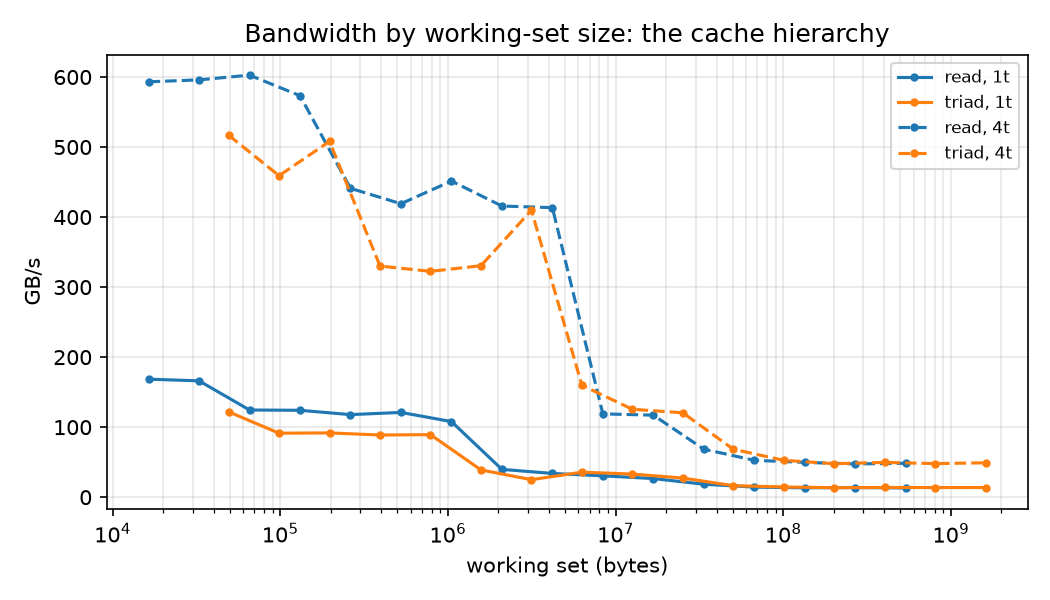
\includegraphics[width=0.92\linewidth]{bandwidth_sweep.png}
\caption{本机读带宽（蓝）与 triad（橙）随工作集的变化；实线 1 线程，虚线 4 线程。triad 的横轴是三个数组之和，所以起点是 48 KiB。}\label{fig:sweep}
\end{figure}

\begin{table}[H]
\centering\small
\caption{本机带宽阶梯（\texttt{roofline.jsonl}，每点 11 次中位数）}\label{tab:ladder}
\begin{tabular}{lrrl}
\toprule
工作集 & 1 线程只读 GB/s & 4 线程只读 GB/s & 所在层（推断） \\
\midrule
16--32 KiB & 166--169 & 593--596 & L1（48 KiB/核） \\
64 KiB--1 MiB & 108--125 & 419--603 & L2（1.25 MiB/核；4 线程时共 5 MiB） \\
2--16 MiB & 27--40 & 117--416 & L3（共享；4 线程到 4 MiB 仍在各核 L2） \\
32 MiB & 18.5 & 68.6 & L3 → DRAM 过渡 \\
128--512 MiB & 13.2--13.8 & 47.5--49.7 & DRAM \\
\bottomrule
\end{tabular}
\end{table}

读 \cref{fig:sweep}：1 线程蓝实线有三个清楚的台阶。32 KiB 到 64 KiB 从 166 掉到 125（出 L1），1 MiB 到 2 MiB 从 108 掉到 40（出 L2），
之后在 L3 区间缓慢下滑（34、31、27 GB/s），32 MiB 是 18.5，到 128 MiB 以后稳定在 13.2--13.8。L1 到 DRAM 差 12 倍（166 / 13.4）。
4 线程蓝虚线的台阶位置右移：L2 平台一直延长到 4 MiB（413 GB/s），8 MiB 才掉到 119。原因是每个线程只扫自己的 1/4，
4 MiB 总工作集每核只有 1 MiB，仍在 1.25 MiB 的 L2 里。所以“L2 带宽”和“L2 容量”都不是一个数，它们依赖有多少核在用各自的 L2。

triad（橙）在 DRAM 区间 1 线程 13.8 GB/s、4 线程 49.1 GB/s（按 3 个流计），与只读核几乎相同；在缓存区间低于只读核，因为每个元素多一次写。
4 线程 triad 在 393 KiB--1.5 MiB 有一段约 330 GB/s 的凹陷、3 MiB 又回到 410，这个非单调没有解释，结论不依赖它。

\begin{findingbox}[：同一个 kernel 换个工作集就换了一条屋顶]
1 线程从 L1 供数时 fp32 拐点只有 $154.9/166 = 0.93$ FLOP/B，从 DRAM 供数时是 11.5 FLOP/B，差 12 倍。
分块好、数据驻留 L1 的 kernel 几乎都在拐点右边（计算受限）；没有分块、每次都从 DRAM 取数的同一个 kernel 则可能在左边。
阶梯的台阶位置（本机 1 线程 32 KiB、1 MiB）直接告诉你分块该切多大。
\end{findingbox}

\subsection{单核喂不满 DRAM}\label{sec:triad}

\begin{table}[H]
\centering\small
\caption{DRAM 区间：只读与 triad（\texttt{summary.json}）}\label{tab:triad}
\begin{tabular}{lrrrr}
\toprule
线程 & 只读 GB/s & triad（3 流）GB/s & triad × 4/3（含写分配） & 只读 / 4 线程只读 \\
\midrule
1 & 13.4 & 13.8 & 18.4 & 28\% \\
4 & 48.4 & 49.1 & 65.5 & 100\% \\
\bottomrule
\end{tabular}
\end{table}

1 线程只读 13.4 GB/s，只有 4 线程 48.4 GB/s 的 28\%；4 线程是 1 线程的 3.61 倍，接近线性，说明 4 个核还没有把总线占满。
按 \cref{eq:wa}，1 线程 triad 在总线上的流量是 $13.8 \times 4/3 = 18.4$ GB/s，比同一个核的只读高 37\%：同一个核挂两个读流、一个写流时在途 miss 更多，带宽就更高。
这与 \cref{eq:e2} 的预测一致——单核 13.4 GB/s 是单核在途请求数的上限，不是总线的上限。
同一结论在 M08（块量化 decode）里也出现：fp32 GEMV（4096×4096，64 MiB 权重）同时读多行，4 线程 58.1 GB/s，高于同样 64 MiB 工作集下只读核的 52.7 GB/s。

\begin{iqbox}{为什么单核只有 13.4 GB/s，4 核却有 48.4？是总线太窄吗？}
不是。按 Little 定律~\cite{little}（\cref{eq:e2}），持续带宽 = 在途字节 / 延迟。每个核能挂起的 L1 miss 数是固定的（十几个 fill buffer 加 L2 预取），
延迟取 100 ns 时 13.4 GB/s 对应约 21 条 cache line 在途；4 核 48.4 GB/s 对应每核约 19 条，每核在途数没变，所以总带宽随核数近乎线性（3.61 倍）。
两个旁证：triad 按写分配计有 18.4 GB/s，比同一个核的只读多 37\%；加线程有效、加 SIMD 宽度无效。
所以单核受的是延迟和并发度的限制，不是总线宽度。工程含义：单线程 LLM decode 的速度上限是“单核带宽 / 权重字节”，不是“总线峰值 / 权重字节”。
\\[2pt]\textbf{常见错答：}“单核带宽低是因为内存总线窄 / DDR 频率低。”这解释不了 4 核为什么能到 3.6 倍。
\end{iqbox}

%=====================================================================
\section{结果二：峰值与拐点}\label{sec:peaks}

\begin{table}[H]
\centering\small
\caption{本机屋顶（\texttt{summary.json}）}\label{tab:peaks}
\begin{tabular}{lrrr}
\toprule
 & 1 线程 & 4 线程 & 4 线程 / 1 线程 \\
\midrule
fp32 FMA（16 链 \texttt{vfmadd} zmm） & 154.9 GFLOP/s & 596.6 & 3.85 \\
int8 VNNI（16 链 \texttt{vpdpbusd} zmm） & 396.1 GOP/s & 1492.7 & 3.77 \\
DRAM 只读 & 13.4 GB/s & 48.4 & 3.61 \\
L1 只读 & 166.1 GB/s & 595.9 & 3.59 \\
int8 / fp32 & 2.56 & 2.50 & \\
fp32 拐点 & 11.5 FLOP/B & 12.3 & \\
int8 拐点 & 29.5 op/B & 30.8 & \\
\bottomrule
\end{tabular}
\end{table}

4 线程时算力与带宽几乎同比放大（fp32 3.85 倍，DRAM 3.61 倍），拐点基本不变（11.5 → 12.3）。这是因为 4 个核还没把 DRAM 总线占满；
核再多，带宽会先饱和，拐点会右移——这在服务器上得到验证（\cref{sec:xeon}）。
4 线程每核 fp32 149.1 GFLOP/s，比 1 线程低 4\%，对应 2.42 → 2.33 GHz 的全核 AVX-512 降频（\cref{sec:peakderiv}）。
L1 读每核 149 GB/s，同样比 1 线程的 166 低约 10\%。

\subsection{int8 为什么只有 2.56 倍}

代入 \cref{eq:int8ratio}：
\begin{align}
\frac{P_{\text{int8}}}{P_{\text{fp32}}} &= \frac{396.1}{154.9} = 2.56 \quad(\text{位宽推出 } 4), \notag\\
\text{VNNI 条/周期} &= \frac{396.1\times 10^{9}}{128 \times 2.42\times 10^{9}} = 1.28 \quad(\text{FMA 是 2}). \notag
\end{align}
int8 的指令吞吐只有 FMA 的 64\%。这可能来自端口分配（\texttt{vpdpbusd} 能发到的端口少于 FMA），也可能来自频率档位（重 int8 负载的降频更深）；
只看墙钟时间无法区分，要靠性能计数器或 uops.info 的表，这台 VM 两者都没有。工程结论不依赖原因：int8 的算力屋顶必须单独量，
按 fp32 × 4 画会把 int8 拐点高估 $4/2.56 = 1.56$ 倍，把一些实际受算力限制的 int8 kernel 错判为受带宽限制。

\begin{iqbox}{int8 比 fp32 快多少？为什么不是 4 倍？}
峰值上本机 2.56 倍、Xeon 8470Q 上 2.66 倍，都不是 4 倍。VNNI 一条 \texttt{vpdpbusd} 做 64 个乘加（128 op），一条 FMA 做 16 个（32 FLOP），
位宽推出 4 倍的前提是两种指令每周期发射数相同；实测按 2.42 GHz 折算 VNNI 每周期 1.28 条，FMA 2 条，吞吐只有 64\%。
实际 kernel 还要再打折：requant、打包布局、int32 累加的水平求和都要指令。本仓库 VNNI 打包 GEMM 最高 221 GOP/s，是 int8 峰值的 56\%，
而 fp32 AVX-512 GEMM 是 28--41 GFLOP/s，kernel 层面最多差 5 倍多，但那是因为 fp32 GEMM 写得更差，不是 int8 本身更快。
\\[2pt]\textbf{常见错答：}“int8 位宽是 fp32 的 1/4，所以算力是 4 倍。”另一个常见错是用厂商 TOPS 当峰值，TOPS 常含 2:4 稀疏。
\end{iqbox}

\begin{iqbox}{某芯片宣称 8 核 3 GHz、AVX-512 单 FMA 端口、fp32 峰值 3 TFLOP/s，可信吗？}
按 \cref{eq:peak}：$8 \times 3\times10^{9} \times 1 \times 16 \times 2 = 0.77$ TFLOP/s。要到 3 TFLOP/s 需要 4 个 512 位 FMA 端口，或者 12 GHz，都不现实，声明不可信。
本实验用同样的方法自检：1 线程 154.9 GFLOP/s 反推 2.42 GHz（双端口）合理，若按单端口则是 4.84 GHz，不可能；
Xeon 上 232 GFLOP/s 反推 3.6 GHz，与单核睿频相符。反推出的频率或端口数不合理，要么声明错，要么测量错（例如累加链太少、被编译器消掉）。
\end{iqbox}

%=====================================================================
\section{结果三：把 kernel 放上屋顶}\label{sec:kernels}

\begin{figure}[H]
\centering
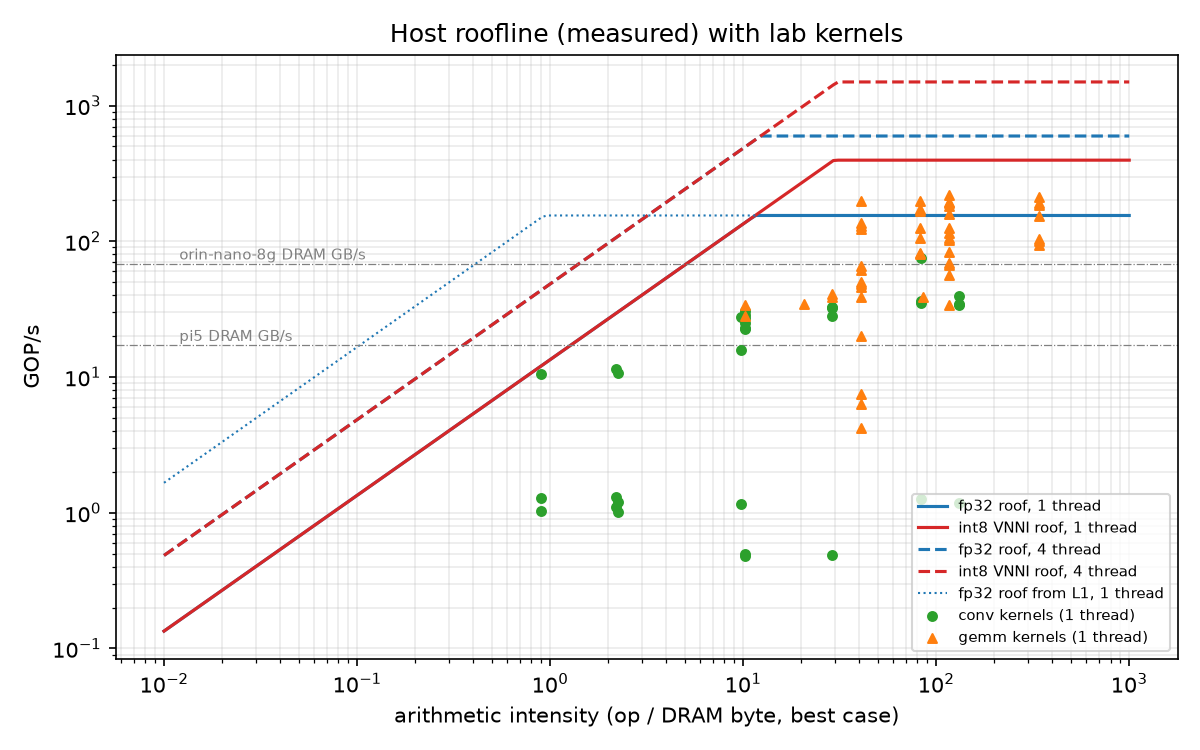
\includegraphics[width=0.95\linewidth]{roofline.png}
\caption{本机实测屋顶与各 lab kernel（均为 1 线程）。蓝：fp32 屋顶，红：int8 VNNI 屋顶；实线 1 线程，虚线 4 线程；蓝色点线是从 L1 供数的 fp32 屋顶。
绿点是 conv-kernels 的卷积，橙色三角是 int8-kernels 的 GEMM。两条灰色点划线是 Pi 5（17.1 GB/s）与 Orin Nano（68 GB/s）数据手册的 DRAM 总线带宽，不是实测。}\label{fig:roofline}
\end{figure}

读 \cref{fig:roofline}：横轴是 \cref{eq:e3gemm,eq:e3conv} 的最好情况强度，纵轴 GOP/s，都是对数坐标，两条屋顶在其中都是直线。
1 线程 fp32 屋顶在 11.5 FLOP/B 处折平，int8 屋顶在 29.5 op/B 处折平；4 线程两条屋顶整体上移约 3.6--3.9 倍，拐点几乎不动。
从 L1 供数的屋顶在 0.93 FLOP/B 就折平，说明只要数据在 L1，几乎所有点都应当是计算受限。
绿点在纵向上分成三层：$10^{0}$ 附近一层是朴素 NCHW 与通用 CHW depthwise（约 0.5--1.3 GFLOP/s），10--40 GFLOP/s 一层是各种 GEMM 化卷积与 NHWC depthwise，
最高的是 Winograd~\cite{lavin2016}（等效 75 GFLOP/s）。没有点越过屋顶；点若画在屋顶上方，说明强度算错了（数据实际命中了更快的一层，或者漏算了某个张量的流量）。

\begin{table}[H]
\centering\small
\caption{代表性卷积 kernel 的效率（1 线程 fp32，\texttt{lab\_points.csv}；效率按 \cref{eq:eff}，$\beta = 13.4$ GB/s，$P_{\text{peak}} = 154.9$）}\label{tab:kernels}
\begin{tabular}{lrrrr}
\toprule
kernel & 强度 FLOP/B & 屋顶 GFLOP/s & 实测 GFLOP/s & 效率 \\
\midrule
depthwise 3×3 s2，NHWC SIMD & 0.90 & 12.0 & 10.4 & 0.87 \\
depthwise 3×3 56×56，NHWC SIMD & 2.25 & 30.1 & 10.8 & 0.36 \\
depthwise 3×3 14×14，NHWC SIMD & 2.20 & 29.5 & 11.4 & 0.39 \\
1×1 expand 56×56，pointwise GEMM & 10.2 & 137.1 & 30.5 & 0.22 \\
1×1 project 56×56，pointwise GEMM & 10.2 & 137.1 & 27.2 & 0.20 \\
stem 3×3 224，implicit GEMM & 9.80 & 131.5 & 27.8 & 0.21 \\
ResNet 3×3 56×56，implicit GEMM & 131.9 & 154.9 & 34.3 & 0.22 \\
ResNet 3×3 56×56，Winograd F(2,3)（等效） & 131.9 & 154.9 & 39.7 & 0.26 \\
ResNet 3×3 14×14，Winograd F(2,3)（等效） & 83.8 & 154.9 & 75.0 & 0.48 \\
同层（ResNet 3×3 14×14）朴素 NCHW & 83.8 & 154.9 & 1.3 & 0.008 \\
\bottomrule
\end{tabular}
\end{table}

\begin{itemize}
  \item \textbf{带宽受限的点离屋顶最近}。depthwise 的强度只有 0.9--2.25 FLOP/B，屋顶是斜线；NHWC SIMD 实现到 36--87\%，stride 2 的那一层最接近（输出少、读入每字节摊到的指令少）。
  同一层的朴素 NCHW 与通用 CHW 实现只有 3--11\%（\texttt{lab\_points.csv} 中 0.034--0.106）：布局不对时连带宽屋顶都碰不到。
  \item \textbf{GEMM 类卷积离两条屋顶都远}。1×1 卷积 56×56 的强度 10.2 FLOP/B 落在拐点 11.5 稍左，屋顶 137 GFLOP/s，实测最快 30.5，效率 22\%。
  它不是“受带宽限制”——离斜线和平线都差 4 倍以上，瓶颈是 kernel 本身：教学 GEMM 没有寄存器分块与打包。除 stem 层的 im2col（12\%）外，所有 im2col / implicit / pointwise GEMM 都在 16--26\% 之间。
  \item \textbf{Winograd 的效率是“等效”的}。它按直接卷积的 FLOP 计数，实际乘法少 2.25 倍，所以 14×14 层能到 48\%；在 56×56 层只有 26\%，变换开销没有摊平。
  \item \textbf{朴素 NCHW 不到 1\%}：同一个 ResNet 3×3 14×14 层，1.3 对 75.0 GFLOP/s，差 60 倍。
\end{itemize}

\subsection{int8 GEMM 的点}

橙色三角的强度按 int8 字节计（\cref{eq:e3gemm} 取 $b=1$），只能对照 int8 屋顶，所以 \texttt{lab\_points.csv} 里它们的 \texttt{eff} 为空；
fp32\_avx512 的点按 4 字节计，强度是同形状 int8 点的 1/4。下表按 \cref{eq:eff} 用 int8 屋顶手算（强度都在 29.5 op/B 右边，屋顶取 396.1）：

\begin{table}[H]
\centering\small
\caption{int8-kernels 的 GEMM（1 线程，GOP/s；括号内为 int8 峰值 396.1 的比例）}\label{tab:gemm}
\begin{tabular}{lrrrr}
\toprule
形状 & int8 强度 op/B & fp32 AVX-512 & VNNI 打包 & 打包 + 融合 requant \\
\midrule
mbv2 pw expand 56（K = 24） & 40.9 & 33.8 & 129.0（33\%） & 66.0（17\%） \\
mbv2 pw project 56 & 40.9 & 28.3 & 198.6（50\%） & 135.3（34\%） \\
mbv2 pw expand 14 & 115.9 & 38.7 & 182.0（46\%） & 125.6（32\%） \\
mbv2 pw project 14 & 115.9 & 40.6 & 220.6（56\%） & 196.4（50\%） \\
mbv2 pw head 7 & 82.3 & 34.3 & 199.0（50\%） & 171.9（43\%） \\
square 512 & 341.3 & 39.2 & 211.8（53\%） & 190.8（48\%） \\
\bottomrule
\end{tabular}
\end{table}

VNNI 打包 GEMM 最高 221 GOP/s（56\%），square 512 是 212（53\%）。在 \cref{fig:roofline} 上，K = 24 那一组三角在 41 op/B 处从 4 GOP/s（未打包的逐点积 VNNI）
一直拉到 129 GOP/s（打包），纵向跨度 30 倍，强度完全相同：这是“强度相同、kernel 不同”的最直观例子。
把 requant 融合进 epilogue 后每个形状都掉一截，K = 24 时从 129 掉到 66：K 小时每个输出分到的乘加少，epilogue 的固定成本占比大。

\begin{findingbox}[：先看在拐点哪一侧，再决定往哪个方向改]
depthwise（0.9--2.25 FLOP/B）在拐点左边，NHWC SIMD 已经到 36--87\%，再优化只能减字节（融合、量化、换布局）；
ResNet 3×3（84--132 FLOP/B）在右边，GEMM 实现只到 16--26\%，缺的是寄存器分块与打包，这是 M06 调度搜索要解决的；
1×1 卷积（10.2）在拐点附近却离两条屋顶都远 4 倍以上，说明“效率低就是带宽受限”是错误的归因。
\end{findingbox}

\begin{iqbox}{屋顶下面的点离屋顶很远，怎么办？}
看它在拐点哪一侧。左边先减字节：算子融合（少一次中间张量往返）、量化（每参数字节减半）、换布局（NHWC 让 depthwise 连续读）、提高复用。
右边先喂满 SIMD：寄存器分块（让每次加载服务多个 FMA）、打包（让内层循环连续、无 gather）、去掉水平求和。
本机 1×1 卷积 30 GFLOP/s 离 137 的屋顶很远，强度在拐点附近，两种方向都不是主因，缺的是寄存器分块；int8 GEMM 打包前后在同一强度上差 30 倍，也说明布局比字节更关键。
如果点在屋顶上方，先怀疑强度：数据命中了 L1/L2 而你按 DRAM 计，或漏算了某个张量。
\end{iqbox}

\begin{iqbox}{LLM decode 为什么慢？在本机上怎么估？}
decode 每 token 每个权重只用一次，是 GEMV。按 \cref{eq:e3gemv}，强度约为 $2/b_w$：Q4\_0 每参数 0.5625 B，约 3.6 FLOP/B，远在 11.5 的拐点左边，
所以时间约等于“权重字节 / 持续带宽”。0.5 B 参数的模型 Q4\_0 只计权重约 0.28 GB：本机 1 线程 $0.28/13.4 \approx 21$ ms/token，4 线程约 5.8 ms；
若拿 Pi 5 数据手册的 17.1 GB/s 算是 16.5 ms，但那是总线算术，单个 A76 核实际更慢。
关键是用单核或所用核数的\emph{实测}带宽去除，而不是总线峰值——llama-cpp-7b 报告里 Xeon 单线程解码 Qwen2.5-7B Q4\_0 正好到单核 DRAM 读的 93\%。
\end{iqbox}

%=====================================================================
\section{结果四：服务器重跑，Xeon 8470Q 1--16 线程}\label{sec:xeon}

命令为 \texttt{EDGE\_THREADS=1,2,4,8,16 python scripts/run\_experiments.py --max-mib 2048}，\texttt{taskset} 绑 NUMA1 的 16 个物理核（60--75），
工作集扫到 2 GiB 以越过 105 MB 的 L3。原始数据在 \nolinkurl{artifacts/raw/xeon8470q/}。

\begin{table}[H]
\centering\small
\caption{Xeon 8470Q 屋顶随线程数（\texttt{xeon8470q/summary.json}）}\label{tab:xeon}
\begin{tabular}{rrrrrrrr}
\toprule
线程 & \makecell{L1 读\\GB/s} & \makecell{DRAM 读\\GB/s} & \makecell{triad\\GB/s} & \makecell{fp32\\GFLOP/s} & \makecell{int8\\GOP/s} & \makecell{int8 /\\fp32} & \makecell{fp32 拐点\\FLOP/B} \\
\midrule
1 & 277 & 17.5 & 19.9 & 232 & 617 & 2.66 & 13.3 \\
2 & 555 & 33.4 & 37.1 & 375 & 1176 & 3.13 & 11.2 \\
4 & 1045 & 66.6 & 72.3 & 939 & 2457 & 2.62 & 14.1 \\
8 & 2311 & 120.6 & 112.7 & 1712 & 4806 & 2.81 & 14.2 \\
16 & 3515 & 193.5 & 157.8 & 3167 & 9208 & 2.91 & 16.4 \\
\bottomrule
\end{tabular}
\end{table}

\begin{figure}[H]
\centering
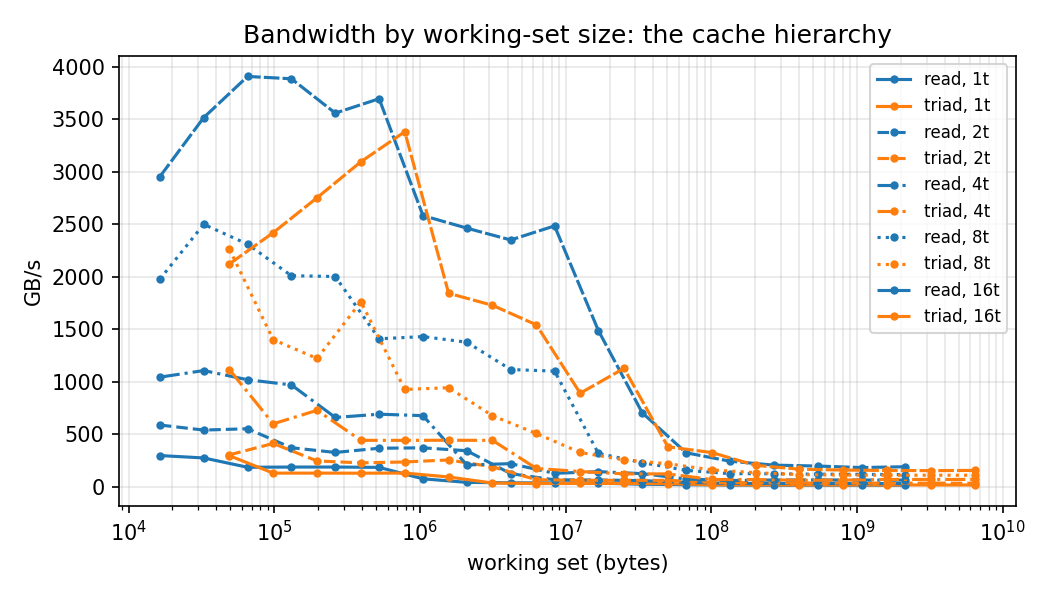
\includegraphics[width=0.92\linewidth]{xeon8470q/bandwidth_sweep.png}
\caption{Xeon 8470Q 读（蓝）与 triad（橙）带宽随工作集，1--16 线程（线型区分线程数）。线性纵轴把 DRAM 段压在底部，台阶结构见 \cref{fig:scaling} 的对数纵轴。}\label{fig:xeonsweep}
\end{figure}

读 \cref{fig:xeonsweep}：线性纵轴下，多线程的缓存段从约 300 GB/s（1 线程）到 3906 GB/s（16 线程，64 KiB 总工作集）展开，
而所有曲线在 $10^{8}$ 字节以后都挤在 200 GB/s 以下——缓存带宽随核数线性放大，DRAM 带宽放大得少得多，这是本节最重要的形状。
16 线程 triad（橙）的缓存段在三个数组合计 768 KiB 处达到 3380 GB/s，与只读的峰值同量级。DRAM 段 16 线程 triad 157.8 GB/s 低于只读 193.5，与本机“两者几乎相同”的形状不同，见 \cref{sec:throttle}。

\begin{figure}[H]
\centering
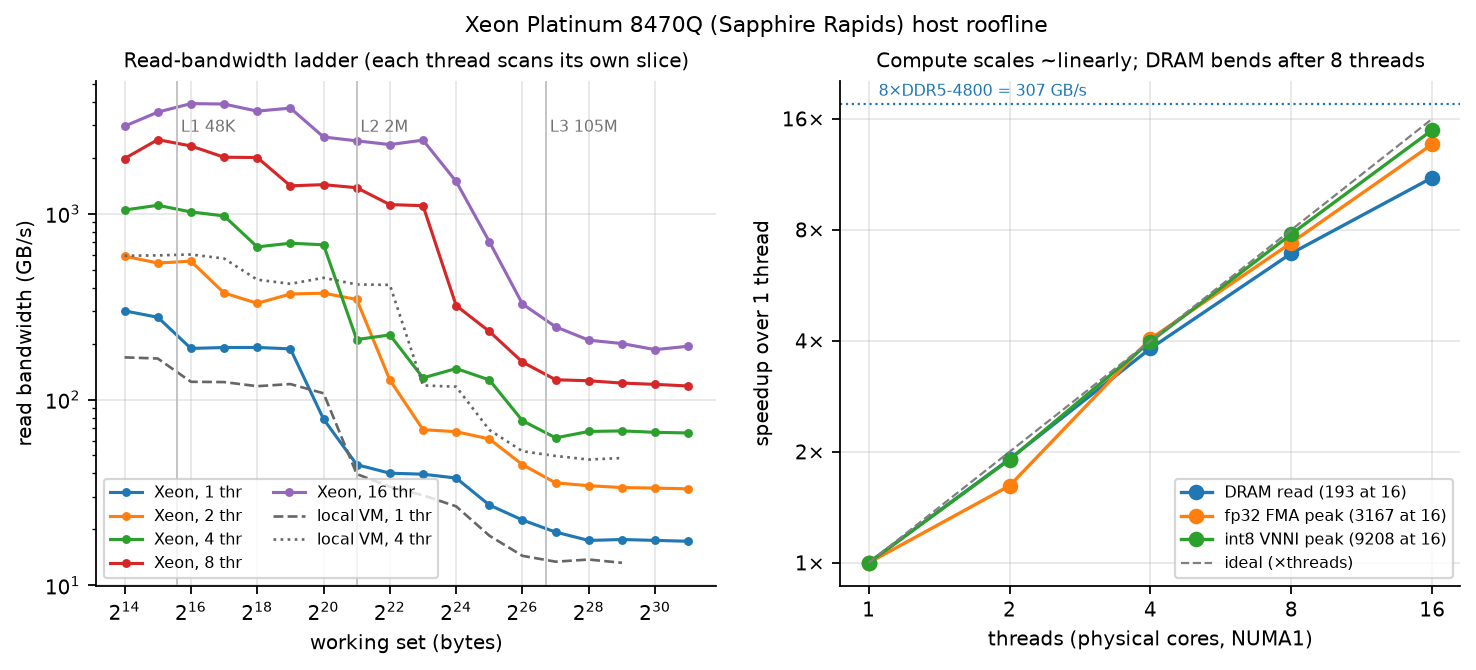
\includegraphics[width=\linewidth]{xeon8470q/thread_scaling.png}
\caption{左：每个线程数的读带宽阶梯（对数纵轴；竖线标出 L1 48K、L2 2M、L3 105M；灰色虚线 / 点线为本地 VM 的 1 / 4 线程）。
右：16 线程内 DRAM 读、fp32 峰值、int8 峰值相对 1 线程的加速比，灰色虚线是理想的“× 线程数”，顶部蓝色点线标出 8 × DDR5-4800 = 307 GB/s。}\label{fig:scaling}
\end{figure}

读 \cref{fig:scaling}：
\begin{itemize}
  \item \textbf{右图}：fp32 与 int8 峰值贴着理想对角线（16 线程分别 13.7 倍与 14.9 倍），DRAM 读在 8 线程后离开对角线，16 线程只有 11.1 倍（193.5 / 17.5）。
  8 → 16 线程 DRAM 只涨 1.6 倍（120.6 → 193.5）。这就是“加核让 GEMM 变快，但让 GEMV 变快得少”的图形版本。
  2 线程的 fp32 只有 1 线程的 1.6 倍，是右图里唯一明显低于对角线的计算点，可能被限流（\cref{sec:throttle}）。
  \item \textbf{左图}：台阶位置随线程数右移。1 线程在 512 KiB → 1 MiB 处从 187 掉到 78，16 线程要到 8 MiB → 16 MiB 才从 2484 掉到 1488（每线程 1 MiB），
  因为每线程扫自己的切片，16 线程时总工作集要到 16 倍才出各核 L2。“L2 带宽”不是一个数，它依赖多少核在用 L2。
  \item \textbf{左图灰线}：本地 VM 的 1 线程曲线在 DRAM 段（$2^{27}$ 以后）与服务器 1 线程几乎重合（13.4 对 17.5 GB/s）：两代服务器 CPU 的单核访存能力差不多。
\end{itemize}

\begin{table}[H]
\centering\small
\caption{Xeon 8470Q 1 线程与 16 线程的读带宽阶梯（\texttt{xeon8470q/roofline.jsonl}）}\label{tab:xeonladder}
\begin{tabular}{lrlrl}
\toprule
1 线程工作集 & GB/s & & 16 线程工作集 & GB/s \\
\midrule
16--32 KiB & 277--300 & & 16 KiB--512 KiB & 2953--3906 \\
64--512 KiB & 187--191 & & 1--8 MiB & 2351--2583 \\
1 MiB & 78.4 & & 16 MiB & 1488 \\
2--16 MiB & 37.8--44.6 & & 32 MiB & 707 \\
32--128 MiB & 19.4--27.1 & & 64--128 MiB & 246--326 \\
256 MiB--2 GiB & 17.3--17.7 & & 256 MiB--2 GiB & 185--208 \\
\bottomrule
\end{tabular}
\end{table}

\begin{figure}[H]
\centering
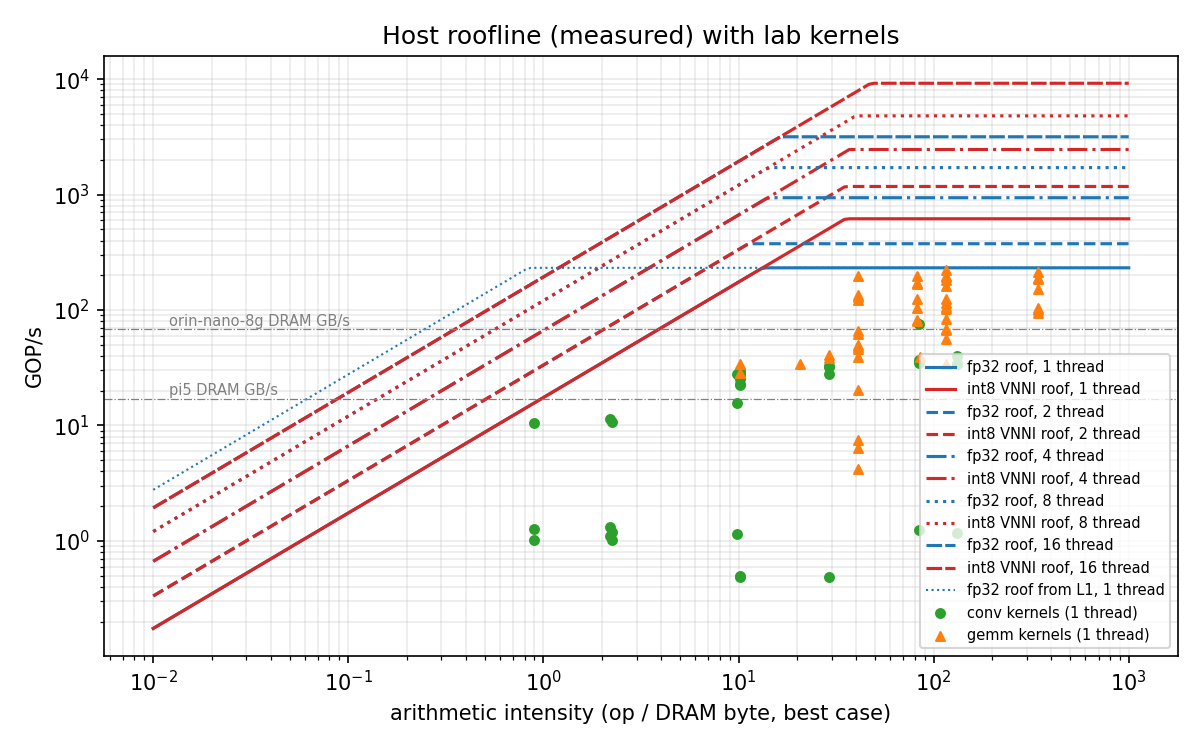
\includegraphics[width=0.95\linewidth]{xeon8470q/roofline.png}
\caption{Xeon 8470Q 的实测屋顶（1--16 线程，蓝 fp32、红 int8，线型区分线程数）。图中 kernel 点与 \cref{fig:roofline} 完全相同，是本地 VM 上测得的 1 线程结果，只用于对照屋顶的位置。}\label{fig:xeonroof}
\end{figure}

读 \cref{fig:xeonroof}：五对屋顶的斜段彼此平行（斜率都是 1），从 1 线程到 16 线程上移约 11 倍；平段上移更多（fp32 13.7 倍、int8 14.9 倍），
所以折点（拐点）随线程数右移：fp32 13.3 → 16.4 FLOP/B，int8 35.3 → 47.6 op/B。
1 线程 fp32 屋顶的拐点 13.3 与本机的 11.5 接近，图中绿点相对屋顶的位置与 \cref{fig:roofline} 大致相同；
注意 \texttt{xeon8470q/lab\_points.csv} 中的 GOP/s 与本机文件逐行相同，只有 \texttt{eff} 按 Xeon 屋顶重算（例如 depthwise s2 从 0.87 变成 0.67），
那不是服务器上的效率，因为这些 kernel 没有在服务器上用这个脚本重测。

\begin{findingbox}[：DRAM 带宽 16 线程仍未饱和，但已开始弯曲]
16 线程 193.5 GB/s 是“1 线程 × 16”（279 GB/s）的 69\%，是单插槽 8 × DDR5-4800 理论值 307 GB/s 的 63\%。
本机 4 线程时“随核数近乎线性”的观察在 8 线程后开始弯曲（8 → 16 只涨 1.6 倍），而计算峰值仍近乎线性，所以拐点随线程数上升：13.3 → 16.4 FLOP/B。
多核让更多的层变成带宽受限：一个 14 FLOP/B 的 kernel 在 1 线程时计算受限，在 16 线程时受带宽限。
\end{findingbox}

按 \cref{eq:e2} 再看每核在途数（延迟仍按 100 ns 假设，未实测）：1 线程 17.5 GB/s 约 27 条 line，8 线程 120.6 GB/s 每核约 24 条，16 线程 193.5 GB/s 每核约 19 条。
若每核能挂起的 miss 数不变，每核带宽下降就意味着负载下的延迟上升——接近饱和时排队变长，这是弯曲的一种解释，没有延迟测量支撑。

\begin{iqbox}{服务器内存带宽有几百 GB/s，为什么单线程解码 7B 模型还是很慢？}
几百 GB/s 是整个插槽所有内存通道被很多核同时拉满时的数字。单线程只能靠自己核里的十几个在途请求取数据，按 \cref{eq:e2}，
延迟 100 ns 量级时上限就是二十 GB/s 左右；Xeon 8470Q 实测 17.5 GB/s，比 4 核 VM 的 13.4 只高 30\%——SPR 的 mesh 更大、跨 mesh 延迟更长，核多了总带宽才上去。
所以单线程 decode 测的就是单核带宽：llama-cpp-7b 报告里 Q4\_0 单线程 3.97 tok/s × 每 token 4.1 GB = 16.3 GB/s，是单核 DRAM 读的 93\%；16 线程才有 37.4 tok/s。
要让 decode 变快，先加线程把在途请求数堆上去，再减每 token 的字节。
\end{iqbox}

\subsection{频率与 int8 比值}

1 线程 fp32 232 GFLOP/s，按 \cref{eq:peak} 反推 $232/64 = 3.6$ GHz（单核睿频）；16 线程每核 198 GFLOP/s，对应 3.1 GHz（多核 AVX-512 降频）。
按 \cref{eq:int8ratio}，1 线程 VNNI 每周期 $617.2 / (128 \times 3.6) \approx 1.34$ 条，与本机的 1.28 接近：
两代核心上 VNNI 的指令吞吐都约为 FMA 的三分之二，int8 / fp32 稳定在 2.5--2.9 倍（2 线程的 3.13 是 fp32 偏低造成的，见下）。

\subsection{测量干扰}\label{sec:throttle}

这台机器的 cgroup 只给 22 个 CPU 的配额，宿主上还有别的租户（load average 约 12）。两个数字可能是被限流的结果：
2 线程的 fp32 只有 1 线程的 1.6 倍（因此 2 线程 int8 / fp32 达到 3.13、拐点降到 11.2）；16 线程 triad 157.8 GB/s 低于只读 193.5。
后者若按 \cref{eq:wa} 计写分配是 $157.8\times4/3 = 210$ GB/s，高于只读，与本机的形状一致，但这只是一种算术上的可能，不能据此排除限流。
本报告只取单调、可重复的结论。

%=====================================================================
\section{本机与服务器对照}\label{sec:compare}

\begin{table}[H]
\centering\small
\caption{同一份代码、同一组参数，两台机器的屋顶（Xeon / VM 为比值）}\label{tab:compare}
\begin{tabular}{lrrrrrr}
\toprule
 & \multicolumn{3}{c}{1 线程} & \multicolumn{3}{c}{4 线程} \\
\cmidrule(lr){2-4}\cmidrule(lr){5-7}
指标 & VM & Xeon & 比值 & VM & Xeon & 比值 \\
\midrule
L1 读 GB/s & 166.1 & 277.0 & 1.67 & 595.9 & 1045.5 & 1.75 \\
DRAM 读 GB/s & 13.4 & 17.5 & 1.30 & 48.4 & 66.6 & 1.37 \\
triad GB/s & 13.8 & 19.9 & 1.44 & 49.1 & 72.3 & 1.47 \\
fp32 GFLOP/s & 154.9 & 232.0 & 1.50 & 596.6 & 939.3 & 1.57 \\
int8 GOP/s & 396.1 & 617.2 & 1.56 & 1492.7 & 2457.0 & 1.65 \\
int8 / fp32 & 2.56 & 2.66 & & 2.50 & 2.62 & \\
fp32 拐点 FLOP/B & 11.5 & 13.3 & & 12.3 & 14.1 & \\
int8 拐点 op/B & 29.5 & 35.3 & & 30.8 & 36.9 & \\
反推频率 GHz & 2.42 & 3.6 & & 2.33 & -- & \\
\bottomrule
\end{tabular}
\end{table}

\Cref{tab:compare} 把结论分成两类：

\begin{itemize}
  \item \textbf{结构性的，换机器不变}：
  int8 / fp32 都是 2.5--2.7 倍（不是 4 倍）；带宽是一张阶梯，L1 到 DRAM 差一个数量级（VM 12 倍，Xeon 1 线程 16 倍）；
  单核喂不满 DRAM，且 triad 都高于只读（VM 13.8 对 13.4，Xeon 19.9 对 17.5，还未计写分配）；台阶位置随线程数右移；
  conv 与 decode 的强度是算法属性，在两台机器上都分别落在拐点的同一侧（depthwise 与 GEMV 在左，ResNet 3×3 在右）。
  \item \textbf{位置性的，只是本机的常数}：
  拐点的具体值（11.5 对 13.3）；“拐点随线程数基本不变”只在 4 核 VM 上成立，服务器上 8 线程后就右移到 16.4；
  “DRAM 随核数线性”同样只在 4 线程以内成立。凡是强度落在 11--17 FLOP/B 之间的 kernel（如本仓库 1×1 卷积的 10.2、stem 的 9.8 附近），
  换机器或换线程数可能从计算受限变成带宽受限。
\end{itemize}

最值得记住的是比值的排序：计算峰值涨 1.5--1.65 倍、L1 涨 1.7 倍，而 DRAM 只涨 1.3--1.4 倍。服务器“更强”主要强在核多、核快，
单核看到的内存并没有快多少；Pi 5 数据手册的总线峰值 17.1 GB/s 与 Xeon 单核实测的 17.5 GB/s 几乎一样大，这提醒我们端侧芯片的单核持续带宽只会更低，必须在板子上量。

\begin{findingbox}[：单核带宽几乎不随“服务器更强”而提高]
1 线程 DRAM 读 13.4 → 17.5 GB/s，只高 30\%；而 fp32 峰值高 50\%、L1 读高 67\%。按 Little 定律，单核带宽 ≈ 在途 miss × 64 B / 延迟，
每核的 fill buffer 数在两代之间变化不大，SPR 的跨 mesh 延迟还更长，所以单核带宽基本原地踏步，总带宽靠核数堆。
\end{findingbox}

%=====================================================================
\section{测量本身的坑}\label{sec:pitfalls}

\begin{table}[H]
\centering\small
\caption{本实验遇到过的测量错误}\label{tab:pitfalls}
\begin{tabularx}{\linewidth}{>{\raggedright\arraybackslash}p{3.4cm} >{\raggedright\arraybackslash}X >{\raggedright\arraybackslash}p{3.6cm}}
\toprule
问题 & 现象与原因 & 修法 \\
\midrule
每遍扫描都派发线程 & 4 线程 L1 读只测到约 50 GB/s：一次派发几微秒，比扫一遍 16 KiB 长得多，测到的是派发开销 & 线程内重复 reps 遍；自旋线程池（空派发 < 100 µs）；现为 596 GB/s \\
编译器外提重复求和 & 对不变内存反复求和，结果只依赖第一遍，可被提到循环外，带宽虚高 & 每遍后 \texttt{clobber()} \\
累加链太少 & FMA 延迟 4 周期 × 2 端口，少于 8 条链时测到的是延迟而不是吞吐 & 16 条独立链；\texttt{keep()} 防止消除 \\
后台负载 & 一个遗留 Python 进程占一个核 6 天，期间 4 线程数字全部偏低 & 计时前看 CPU 占用；全部重测 \\
cgroup 限流（服务器） & 22 CPU 配额、load average 约 12；2 线程 fp32 与 16 线程 triad 可疑 & 只取单调、可重复的结论 \\
平台检测并级 & 65\% 阈值会把 L2→L3 缓坡并成一级，平台中位数偏离真实 DRAM 值 & 直接取扫描两端各 3 点中位数 \\
\bottomrule
\end{tabularx}
\end{table}

\begin{iqbox}{测内存带宽时，为什么不能在每遍扫描外面套一层 parallel\_for？}
因为派发本身有成本。mlsys-infra M03 在 CS149 A2 上实测过：自旋池 0.78 µs、睡眠池 10.8 µs、每次新建线程 53.3 µs。
16 KiB 在 166 GB/s 下只要约 0.1 µs，派发比要测的东西长一到两个数量级，结果测的是线程池。本实验早期就是这样，4 线程 L1 读约 50 GB/s；
把 reps 次重复放进每个线程内部（一次派发扫约 64 MiB），再换成自旋线程池，同一个测量变成 596 GB/s，差 12 倍。
推广：任何微基准的单次工作量都要远大于框架开销，并且要先测一次“空任务”的开销作为地板。
\end{iqbox}

%=====================================================================
\section{结论}\label{sec:conclusion}

\begin{findingbox}[：本实验的五条结论]
\begin{enumerate}[label=(\arabic*)]
  \item \textbf{屋顶要实测}：本机 1 线程 fp32 154.9 GFLOP/s、int8 396.1 GOP/s、DRAM 13.4 GB/s，拐点 11.5 FLOP/B（int8 29.5 op/B）；4 线程 596.6 / 1492.7 / 48.4，拐点 12.3。
  \item \textbf{int8 不是 fp32 的 4 倍}：实测 2.56 倍（Xeon 2.66），VNNI 每周期 1.28 条对 FMA 2 条；按位宽画 int8 屋顶会把拐点高估约 1.6 倍。
  \item \textbf{单核喂不满 DRAM}：1 线程只读是 4 线程的 28\%，triad 按写分配计 18.4 GB/s 高于只读 13.4，单核受在途请求数限制；Xeon 单核也只有 17.5 GB/s。
  \item \textbf{带宽是阶梯}：L1 166、L2 约 120、L3 27--40、DRAM 13.4 GB/s，L1 到 DRAM 差 12 倍；台阶位置随线程数右移。
  \item \textbf{kernel 的位置决定优化方向}：depthwise NHWC 在斜屋顶下到 36--87\%，GEMM 类卷积在平屋顶下只有 16--26\%，朴素 NCHW 不到 1\%；VNNI 打包 int8 GEMM 最高到 int8 峰值的 56\%。
\end{enumerate}
\end{findingbox}

\subsection*{20 秒讲法}

我在一台 4 核 Ice Lake 虚拟机上用 C++ 微基准量了 roofline：单核 fp32 155 GFLOP/s、int8 VNNI 396 GOP/s，只有 fp32 的 2.56 倍而不是 4 倍；
DRAM 单核只读 13.4 GB/s，只有 4 核的 28\%，因为单核带宽受在途请求数限制，不是总线。拐点 11.5 FLOP/B，所以 depthwise 和 decode 都在带宽一侧，
GEMM 类卷积在算力一侧却只到屋顶的 16--26\%，缺的是寄存器分块。换到 Xeon 8470Q，单核带宽只高 30\%，16 线程 193.5 GB/s 也只有理论值的 63\%，拐点随核数右移到 16.4。

\begin{caveatbox}
\begin{itemize}
  \item 不是任何端侧芯片的屋顶。图里的 Pi 5（17.1 GB/s）和 Orin Nano（68 GB/s）横线是数据手册的总线算术，不是实测；它们的单核持续带宽要在板子上量。
  \item L2 / L3 的容量是推断（虚拟机里 \texttt{Win32\_Processor} 不报 L3），只从阶梯位置读出。
  \item “int8 吞吐只有 FMA 的 64\%”只是墙钟结论；是端口分配还是频率档位，没有性能计数器无法区分。
  \item 4 线程的 DRAM 带宽还没饱和（随核数近乎线性），所以本地的拐点不能外推到更多核；服务器上 8 线程后开始弯曲，16 线程是理论值的 63\%。
  \item Little 定律的在途条数用的是假设的 100 ns 延迟，两台机器都没有测访存延迟；“负载下延迟上升导致弯曲”只是一种解释。
  \item kernel 点的强度是“每个张量只搬一次”的最好情况，真实流量更大，所以表中效率是相对一个偏高屋顶的保守值；Winograd 的效率按直接卷积 FLOP 计，是等效值。
  \item Xeon 屋顶图上的 kernel 点是本地 VM 的测量，\texttt{xeon8470q/lab\_points.csv} 的 \texttt{eff} 不代表服务器上的效率。
  \item 服务器容器有 22 CPU 配额与其他租户，2 线程 fp32 与 16 线程 triad 可能被限流；只读核只有 4 个累加器，L1 读数字是这个 kernel 的值，不一定是加载端口的上限。
\end{itemize}
\end{caveatbox}

%=====================================================================
\section{复现}\label{sec:repro}

\begin{lstlisting}[language=bash]
cd solutions/edge-runtime/host-roofline
python -m pytest -q tests                      # plateaus / ridge / efficiency + C++ smoke test
python scripts/run_experiments.py              # ~20 s, 1 and 4 threads; machine must be idle
python scripts/run_experiments.py --plot-only  # redraw after conv-kernels / int8-kernels reruns

# server rerun (Xeon 8470Q), pinned to 16 physical cores on NUMA1
EDGE_THREADS=1,2,4,8,16 taskset -c 60-75 python scripts/run_experiments.py --max-mib 2048

# the micro-benchmark alone
cpp/bin/roofline-*.exe --mode=bw   --threads=1 --max-mib=512
cpp/bin/roofline-*.exe --mode=fma  --threads=4
cpp/bin/roofline-*.exe --mode=int8 --threads=4
\end{lstlisting}

输出：\nolinkurl{artifacts/raw/roofline.jsonl}（每个工作集大小、每个线程数一行，带 p10/p50/p90 与平台、编译器信息），
\texttt{summary.json}（屋顶与拐点），\texttt{lab\_points.csv}（其他 lab 的 kernel 的强度与效率），图在 \nolinkurl{artifacts/figures/}；
服务器结果在对应的 \texttt{xeon8470q/} 子目录。\texttt{EDGE\_MARCH=haswell} 可强制走 AVX2 分支（\texttt{vpmaddubsw + vpmaddwd}），用于在没有 AVX-512 的机器上复现。


\begin{thebibliography}{99}
\bibitem{roofline} S.~Williams, A.~Waterman, D.~Patterson. Roofline: An Insightful Visual Performance Model for Multicore Architectures. \emph{Communications of the ACM}, 52(4), 2009.
\bibitem{little} J.~D.~C.~Little. A Proof for the Queuing Formula $L=\lambda W$. \emph{Operations Research}, 9(3), 1961.
\bibitem{stream} J.~D.~McCalpin. Memory Bandwidth and Machine Balance in Current High Performance Computers. \emph{IEEE TCCA Newsletter}, 1995.
\bibitem{lavin2016} A.~Lavin, S.~Gray. Fast Algorithms for Convolutional Neural Networks. \emph{CVPR}, 2016.
\end{thebibliography}

\end{document}
